\documentclass{beamer}
\usepackage[utf8]{inputenc}
\usepackage[sorting=none]{biblatex}
\usepackage{tipa, enumerate, parskip, fancyhdr, fmtcount, mathrsfs,
mathtools, nicefrac, amsmath, amsthm, amssymb, tikz, tikz-cd, pgfplots}
\usetikzlibrary{positioning, arrows, calc, decorations.markings,
intersections, pgfplots.fillbetween}
\urlstyle{same}

\addbibresource{histofcurv.bib}

\usetheme{Antibes}
\usecolortheme{beaver}
\setbeamertemplate{enumerate items}[default]
% \setbeamertemplate{bibliography item}[triangle]

\DeclareMathOperator{\Mat}{Mat}
\DeclareMathOperator{\End}{End}
\DeclareMathOperator{\Hom}{Hom}
\DeclareMathOperator{\id}{id}
\DeclareMathOperator{\image}{im}
\DeclareMathOperator{\trace}{tr}
\DeclareMathOperator{\diam}{diam}
\DeclareMathOperator{\Gr}{Gr}
\DeclareMathOperator{\supp}{supp}
\DeclareMathOperator{\GL}{GL}
\DeclareMathOperator{\SL}{SL}
\DeclareMathOperator{\PGL}{PGL}
\DeclareMathOperator{\Ortho}{O}
\DeclareMathOperator{\U}{U}
\DeclareMathOperator{\SO}{SO}
\DeclareMathOperator{\SU}{SU}
\DeclareMathOperator{\sgn}{sgn}
\DeclareMathOperator{\Vol}{Vol}
\DeclareMathOperator{\proj}{proj}
\DeclareMathOperator{\Iso}{Iso}
\DeclareMathOperator{\Aut}{Aut}
\DeclareMathOperator{\Diff}{Diff}
\DeclareMathOperator{\Ad}{Ad}
\DeclareMathOperator{\Span}{span}
\DeclareMathOperator{\Hol}{Hol}

\DeclareMathOperator{\grad}{grad}
\DeclareMathOperator{\diver}{div}
\DeclareMathOperator{\curl}{curl}

\DeclareMathOperator{\dis}{dis}
\DeclareMathOperator{\met}{met}
\DeclareMathOperator{\can}{can}
\DeclareMathOperator{\Lor}{Lor}

\DeclareMathOperator{\Ric}{Ric}
\DeclareMathOperator{\Scal}{Scal}
\DeclareMathOperator{\CAT}{CAT}

\newcommand{\Sphere}{\mathbb{S}}
\newcommand{\Sp}{\mathbb{S}}
\newcommand{\Hy}{\mathbb{H}}
\newcommand{\C}{\mathbb{C}}
\newcommand{\R}{\mathbb{R}}
\newcommand{\Q}{\mathbb{Q}}
\newcommand{\Z}{\mathbb{Z}}
\newcommand{\N}{\mathbb{N}}

\newcommand{\Riem}{\mathcal{R}}
\newcommand{\Met}{\mathcal{M}}

\newcommand{\eps}{\varepsilon}
\newcommand{\norm}[1]{\left\lVert#1\right\rVert}
\newcommand{\transpose}{\intercal}
\newcommand{\hermit}{\mathsf{H}}
\newcommand{\conj}[1]{\bar{#1}}
\newcommand{\abs}[1]{\left|#1\right|}
\newcommand{\partials}[2][]{\frac{\partial #1}{\partial #2}}
\newcommand{\inprod}[2]{\left\langle #1, #2 \right\rangle}

\theoremstyle{definition}
\newtheorem*{exercise}{Bonus Exercise}

\title{The History of Curvature}
\author{Jesse He}
\institute{OSU Reading Classics}
\date{22 March, 2022 (John Marshall White III's Birthday Observed)}

\begin{document}
    
\frame{\titlepage}

\section{The Greeks to the Middle Ages}

\subsection{The Greeks: Aristotle and Apollonius}

\begin{frame}
    \frametitle{Lines Don't Curve; Circles Do}

    Aristotle (384 - 322 BCE) made the astute observation that lines do not curve,
    but circles curve uniformly at each point. Thus, he classified
    plane loci into three categories: linear, circular, and mixed. \cite{unsat-hist}

    Apollonius of Perga (c. 240 BCE - c. 190 BCE) made (implicitly) the first
    calculation of curvature when considering the problem of drawing normal
    segments to conic sections, recognizing that such a normal segment was unique.

\end{frame}

\subsection{Oresme's \textit{Tractatus de configurationibus qualitatum et motuum}}

\begin{frame}
    \frametitle{Nicole Oresme}

    Nicole Oresme (c. 1320 - 1382) was a French philosopher in the Late Middle Ages
    whose \textit{Tractatus de Configurationibus Qualitatum et Motuum} (Treatise
    on the Configurations of Qualities and Motions) contained the first characterization
    of \emph{Curvitas}, noting that the curvature of a circle is inversely proportional
    to its radius. \cite{unsat-hist}

    Attempting to generalize to other curves, Oresme stated that if two curves are tangent
    to a line at the same point from the same side, then the ``smaller'' of the two should
    have more curvature than the larger.

    Oresme's \emph{Tractatus} also contained a number of other important discoveries,
    such as an early use of rectangular coordinates, a computation of geometric series,
    and is credited with the first proof of the divergence of the harmonic
    series. \cite{sep-nicole-oresme}
\end{frame}

\section{Before Calculus}

\subsection{Kepler and Huygens: The Circle of Curvature}

\begin{frame}
    \frametitle{Kepler's Circle of Curvature}

    Johannes Kepler (1571 - 1630) was the first to suggest approximating a curve by
    its \emph{circle of curvature}, the ``closest'' circle to the curve at a point.
    \cite{unsat-hist}

    \begin{figure}
        \centering
        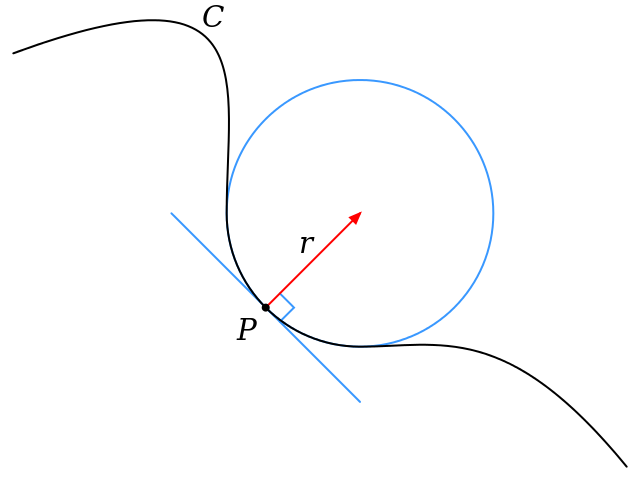
\includegraphics[width=.5\textwidth]{images/Osculating_circle.svg.png}
        \caption{An osculating circle \cite{intern-et-al}}
    \end{figure}
\end{frame}

\begin{frame}
    \frametitle{Huygens' Construction}

    Christiaan Huygens (1629 - 1695) later gave a general way to produce the
    circle of curvature in 1673 in \textit{Horologium Oscillatorium: Sive de Motu Pendulorum
    ad Horologia Aptato Demonstrationes Geometricae}
    (The Pendulum Clock: or Geometrical Demonstrations Concerning the Motion of Pendula as
    Applied to Clocks) using involutes and evolutes.

    Begin with a curve (the \emph{evolute}) whose tangent lines are all on one side,
    and to this attach a flexible string which is pulled taught and then unwound,
    tracing the \emph{involute}.

    Assuming the string is always tangent to the evolute, Huygens shows that it will
    always be normal to the involute, and that the involute and evolute are unique.

\end{frame}

\begin{frame}
    \frametitle{Huygens' Construction (cont.)}

    The radius of curvature of the involute, then, is the distance up the string from
    the involute to the evolute. (Apollonius was unknowingly calculating this in the
    special case of conics.)

    Notice that this requires the \emph{evolute} of the curve to be given in advance.

    Huygens calculated the radii of curvature for some special cases (notably the cycloid)
    and attempts to provide a general method, but was not aware of Newton's and Leibniz's
    calculus and so failed to give a general solution. \cite{unsat-hist}
\end{frame}

\section{The Calculus of Differentiable Curves}

\subsection{Newton and His Contemporaries}

\begin{frame}
    \frametitle{Newton's Method of Fluxions}

    Isaac Newton (1642 - 1727\footnote{Newton died in 1726 according to the Julian calendar,
    but in 1727 according the the Gregorian calendar; since England had not yet adopted the
    Gregorian calendar, Newton's death was recorded as being in 1726 but is usually adjusted
    to 1727 despite his birth usually being listed exclusively by the Julian date.})
    used calculus to describe the center and radius of curvature for a curve at a point
    in Problem V of his posthumously published work \textit{The Method of Fluxions and Infinite
    Series: with its Application to the Geometry of Curve-Lines}. \cite{newton}

    Like Huygens and Kepler, Newton reduces the problem to finding the radius of the osculating
    circle.

\end{frame}

\begin{frame}
    \frametitle{Newton's Method of Fluxions (cont.)}

    \textit{If a Circle touches any Curve on its concave \textesh{}ide, in any given Point,
        and if it be of \textesh{}uch magnitude, that no other tangent Circle can be
        inter\textesh{}cribed in the Angles of Contact near that Point, that Circle
        will be of the \textesh{}ame Curvature as the Curve is of, in that Point of
        Contact. [...]
    }

    \textit{Therefore the Center of Curvature to any Point of a Curve, is the Center of a
        Circle equally curved. And thus the Radius, or Semidiameter of Curvature is
        part of the Perpendicular to the Curve, which is terminated at that Center.
        [...]
    }

    \textit{And the Proportion of Curvature at different Points will be known from
        the Proportion of Curvature of aequi-curve Circles, or from the reciprocal
        Proportion of the Radii of Curvature.
    }
\end{frame}

\begin{frame}
    \frametitle{Newton's Method of Fluxions (cont.)}

    Newton then describes a general method for producing the center of convergence: \cite{newton}

    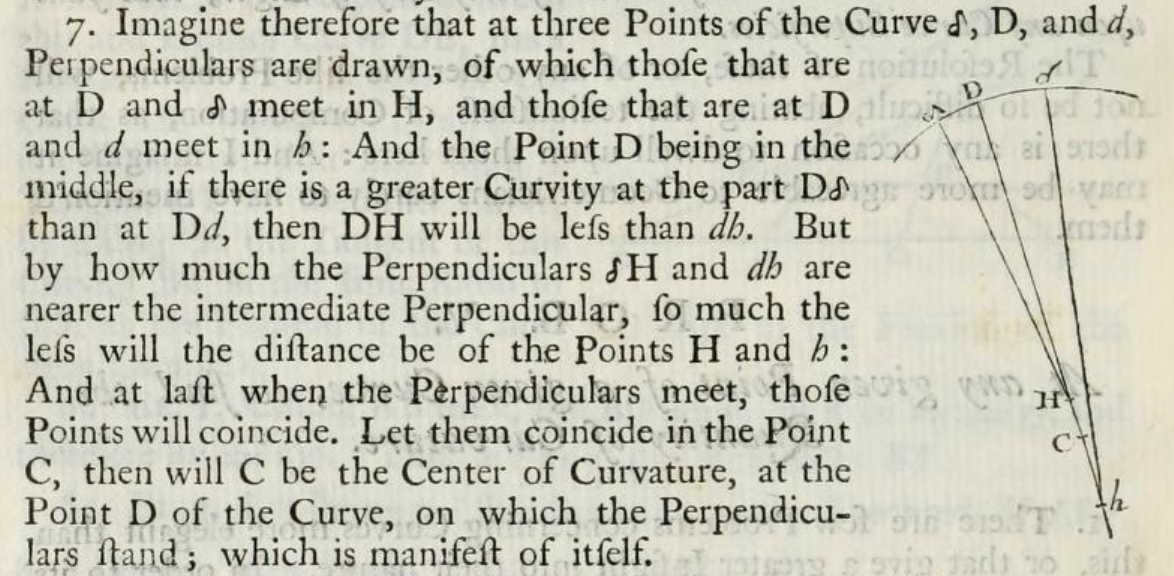
\includegraphics[width=\textwidth]{images/newton-center-construction.png}

    % \textit{Imagine therefore that at three Points of the Curve $\delta$, $D$, and $d$
    %     Perpendculars are drawn, of which tho\textesh{}e that are at $D$ and $\delta$
    %     meet in $H$, and tho\textesh{}e that are at $D$ and $d$ meet in $h$:
    %     And the Point $D$ being in the middle, if there is a greater Curvity at the part
    %     $D\delta$ than at $Dd$, then DH will be le\textesh{}s than dh.
    %     But by how much the Perpendiculars $\delta H$ and $dh$ are nearer the intermediate
    %     Perpendicular, \textesh{}o much the le\textesh{}s will the di\textesh{}tance be of the
    %     Points H and h : And at la\textesh{}t when the Perpendiculars meet, tho\textesh{}e
    %     Points will coincide. Let them coincide in the Point C, then will C be the Center of Curvature,
    %     at the Point D of the Curve, on which the Perpendiculars \textesh{}tand ;
    %     which is manife\textesh{}t of it\textesh{}elf.
    % } \cite{newton}
\end{frame}

\begin{frame}
    \frametitle{Newton's Method of Fluxions (cont.)}

    Using his construction, Newton goes on to show that putting $x = AB$ with
    $\dot{x} = 1$ and $y = BD$ with $z = \dot{y}$ in the following figure \cite{newton}
    the radius of convergence is given by
    \begin{minipage}{.49\textwidth}
        \[
            DC = \dfrac{(1+z^2)^{3/2}}{\dot{z}}
        \]
    \end{minipage}
    \begin{minipage}{.49\textwidth}
        \centering
        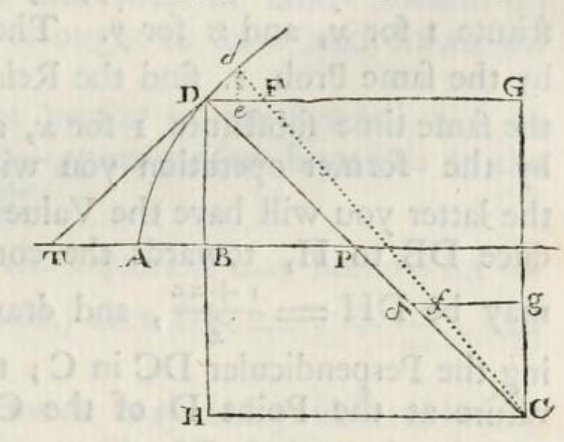
\includegraphics[width=.8\textwidth]{images/newton-formula-derivation.png}
    \end{minipage}
    In modern notation, the radius of curvature of a plane curve $y = y(x)$ is
    \[
        R = \abs{\frac{(1+y'(x)^2)^{3/2}}{y''(x)}}.
    \]
\end{frame}

\begin{frame}
    \frametitle{Newton's Contemporaries}

    Gottfried Wilhelm Leibniz (1646 - 1716) is credited with the term ``osculating circle''
    (or \emph{Circulus Osculans}) in his 1686 paper \textit{Meditation Nova de Natura Anguli
    Contactus et Osculi} (New Meditation on the Nature of Angles of Contact and Osculation).
    \cite{unsat-hist}\cite{geom-diff-view}

    Jacob Bernoulli (1655 - 1705) also worked on the curvature of general
    curves, particularly in his general construction of evolutes from a curve:
    the evolute of a curve $c(t)$ is given by
    \[
        E(t) = c(t) + R(t)n(t)
    \]
    where $R(t)$ is the radius of curvature at $c(t)$ and $n(t)$ is the unit normal
    vector towards the center of curvature.

    Johann Bernoulli (1667 - 1748) also studied curvature, including the radius of curvature
    of a curve in polar coordinates.

\end{frame}

\subsection{Euler and Frenet-Serret: The Second Derivative}

\begin{frame}
    \frametitle{Parameterization by Arc Length}

    Recall that the length of a smooth curve $\gamma : [a,b] \to \R^n$ is given by
    \[
        L(\gamma) = \int_a^b \norm{\dot\gamma(t)} \,dt.
    \]
    Then the \emph{arc length} of $\gamma$ is the function
    \[
        s(t) = \int_a^t \norm{\dot\gamma(t)} \,dt.
    \]
    This is a smooth bijection from $[a,b]$ to $[0,L(\gamma)]$. Writing $t(s)$ for the inverse
    we have the \emph{arc length parameterization} of $\gamma$ by
    \[
      \gamma(s) = \gamma(t(s)).
    \]
    Such a curve has the useful property that $\norm{\dot\gamma(s)} \equiv 1$.
\end{frame}

\begin{frame}
    \frametitle{Euler and the Second Derivative}

    Leonhard Euler (1707 - 1783) proved the following in 1736: \cite{geom-diff-view}

    \begin{theorem}
        Let $\gamma(s)$ be parameterized by arc length. Then the (unsigned) curvature
        $\kappa$ is given by the magnitude of the acceleration:
        \[
          \kappa(\gamma;s) = \norm{\ddot\gamma(s)}.
        \]
    \end{theorem}
\end{frame}

\begin{frame}
    \frametitle{Frenet and Serret}

    Jean Frédéric Frenet (1816 - 1900) and Joseph Alfred Serret (1819 - 1885)
    derived the following formulas in 1847 and 1851:

    \begin{theorem}
        Let $\gamma : [a,b] \to \R^3$ be parameterized by arc length, $T = \dot\gamma$,
        $N = \frac{dT}{ds}/\norm{\frac{dT}{ds}}$, and $B = T \times N$;
        denote the curvature by $\kappa$ and torsion by $\tau$. Then
        \[
            \frac{dT}{ds} = \kappa N, \
            \frac{dN}{ds} = -\kappa T + \tau B, \
            \frac{dB}{ds} = -\tau N.
        \]
    \end{theorem}
    These are the \emph{Frenet-Serret formulas}, and together $T,N,B,\kappa,\tau$
    (the \emph{Frenet-Serret apparatus}) specify $\gamma$ up to rigid motions of $\R^3$.
\end{frame}

\section{Gauss's \emph{Theorema Egregium}}

\subsection{The Curvature(s) of Surfaces}

\begin{frame}
    \frametitle{Surfaces}

    Thus far, we have seen mostly the theory of curves; first in the plane,
    then a generalization in Euclidean 3-space.

    However, the geometry of \emph{surfaces} emerges around Euler's 1760
    paper \textit{Recherches sur la courbure des surfaces} (Research on
    the curvature of surfaces) \cite{geom-diff-view}, and will eventually
    lead to a result of Gauss which would inspire his student Riemann to
    found the modern theory which bears his name.

\end{frame}

\subsection{Gaussian Curvature and the \emph{Theorema Egregium}}

\begin{frame}
    \frametitle{}

    

\end{frame}

\begin{frame}
    \frametitle{Riemann's \textit{Habilitationsvortag}}

    Gauss's \emph{Theorema Egregium} suggests that curvature can
    be studied as an \emph{intrinsic} property of a surface rather than
    the \emph{extrinsic} way in which it is embedded in Euclidean space.

    In addition, the search for a rigorous model of non-Euclidean geometry
    led 

\end{frame}

\section{The Modern Perspective}

\subsection{Manifolds}

\begin{frame}
    \frametitle{Smooth Manifolds}

    \begin{definition}
        A \emph{(topological) $n$-manifold} $M$ is a topological space which is
        locally homeomorphic to $\R^n$. That is, for each $p \in M$ there is
        a neighborhood $U \ni p$ which is homeomorphic to an open subset of $\R^n$.
        We may also require that $M$ be Hausdorff and second countable.
    \end{definition}
    \begin{definition}
        A \emph{smooth structure} (or \emph{atlas}) on $M$ is a collection
        of \emph{charts} $(U_\alpha, \varphi_\alpha)$ such that
        $\varphi_\alpha : U_\alpha \to \R^n$ is a homeomorphism onto its image
        and the \emph{transition functions}
        $\varphi_\alpha \circ \varphi_\beta^{-1} : \R^n \to \R^n$
        are smooth. A topological manifold $M$ endowed with a smooth structure is
        said to be a \emph{smooth} (or \emph{differentiable}) \emph{manifold}.
    \end{definition}
\end{frame}

\begin{frame}
    \frametitle{Riemannian Manifolds}

    \begin{definition}
        To each point $p \in M$ the \emph{tangent space at $p$}, denoted $T_pM$,
        is the vector space of ``directional derivatives'' at $p$. The collection
        of all such tangent spaces, appropriately topologized according to the
        smooth structure of $M$, is the \emph{tangent bundle} $TM$.
    \end{definition}
    \begin{definition}
        A \emph{Riemannian metric} $g$ on a smooth manifold $M$ is a ``smoothly varying''
        inner product $g_p : T_pM \times T_pM \to \R$.
        We say a smooth manifold $M$ endowed with such a metric is a \emph{Riemannian manifold}.
    \end{definition}
\end{frame}

\begin{frame}
    \frametitle{Vector Fields and the Lie Bracket}

    \begin{definition}
        A \emph{(tangent) vector field} $X$ on $M$ is a smoothly varying assignment
        to each $p \in M$ a vector $X_p \in T_pM$. We denote by $\Gamma(TM)$ the
        set of all such vector fields on $M$.
    \end{definition}

    \begin{definition}
        The \emph{Lie bracket} $[X,Y]$ of two vector fields $X, Y \in \Gamma(TM)$
        is the vector field given by
        \[
          [X,Y]f = X(Yf) - Y(Xf)  
        \]
        where we write $Xf$ to mean ``the directional derivative of $f$ in the direction $X$''
        at each point $p \in M$.
    \end{definition}

\end{frame}

\begin{frame}
    \frametitle{The Levi-Civit\`{a} Connection}

    \begin{definition}
        A \emph{connection} on $TM$ is a bilinear map
        \(
            \nabla : \Gamma(TM) \times \Gamma(TM) \to \Gamma(TM)
        \)
        written $(X,Y) \mapsto \nabla_X Y$ such that for any smooth function
        $f : M \to \R$,
        \begin{enumerate}
            \item $\nabla_{fX} Y = f\nabla_XY$
            \item $\nabla_X fY = (\partial_Xf)Y + f\nabla_XY$.
        \end{enumerate}
    \end{definition}
    \begin{theorem}
        Every Riemannian manifold $(M,g)$ has a unique connection $\nabla$
        (the \emph{Levi-Civit\`{a} connection}) which is
        \begin{enumerate}
            \item \textbf{Metric compatible:} $X(g(Y,Z)) = g(\nabla_XY,Z) + g(Y,\nabla_XZ)$
            \item \textbf{Torsion free:} $\nabla_XY - \nabla_YX = [X,Y]$.
        \end{enumerate}
    \end{theorem}
\end{frame}

\subsection{Curvature(s) of a Manifold}

\begin{frame}
    \frametitle{The Curvature Tensor}

    \begin{definition}
        The \emph{curvature tensor} of a Riemannian manifold is the map
        $R : \Gamma(TM) \times \Gamma(TM) \times \Gamma(TM) \to \Gamma(TM)$
        defined by
        \[
          R(X,Y)Z \coloneqq \nabla_X\nabla_YZ - \nabla_Y\nabla_XZ - \nabla_{[X,Y]}Z.  
        \]
    \end{definition}
\end{frame}

\begin{frame}
    \frametitle{An Aside on Holonomy}

    The curvature tensor measures the \emph{holonomy} of a connection,
    or the failure of the \emph{parallel transport} around a loop to preserve
    the direction of a tangent vector, by parallel translating a vector around
    an infinitesimal parallelogram spanned by $X$ and $Y$.
    \begin{figure}
        \centering
        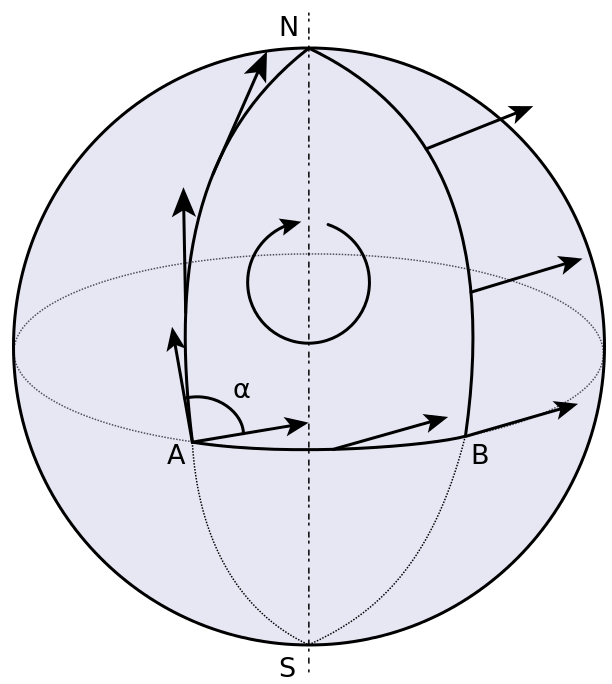
\includegraphics[width=.25\textwidth]{images/Parallel_Transport.svg.png}
        \caption{Holonomy around a geodesic triangle on the sphere.\footnote{Created
        by Fred the Oyster on Wikipedia Commons, used and shared under (CC BY-SA 4.0).}}
    \end{figure}
\end{frame}

\begin{frame}
    \frametitle{An Aside on Holonomy (cont.)}

    The holonomy $\Hol_p(M)$ at a point $p$ forms a \emph{Lie subgroup} of $O(T_pM)$;
    the \emph{restricted holonomy} $\Hol_p^0(M)$ is the subgroup of holonomy considering
    only contractible loops and is related to curvature by the following theorem:
    \begin{theorem}[Ambrose-Singer (1953)]
        The Lie algebra $\mathfrak{hol}_p^0(M) = T_{\id}\Hol_p^0(M)$ is the Lie subalgebra
        of $\End(T_pM)$ generated by $R(v,w)$ for $v, w \in T_pM$.
    \end{theorem}

    Holonomy also gives rise to the remarkable De Rham Decomposition theorem (1952),
    which states roughly that holonomy can be used to locally decompose a simply
    connected manifold as the product of ``nice'' submanifolds, and further that
    this decomposition can be made global if $M$ is complete.
\end{frame}

\begin{frame}
    \frametitle{Ricci and Scalar Curvatures}

    \begin{definition}
        The \emph{Ricci tensor} of a Riemannian manifold is the map
        $\Ric : \Gamma(TM) \times \Gamma(TM) \to C^\infty(M)$ defined by
        \[
            \Ric(Y,Z) \coloneqq \trace(X \mapsto R(X,Y)Z).
        \]
    \end{definition}

    \begin{definition}
        The \emph{scalar curvature} of a Riemannian manifold is the trace of the
        Ricci tensor with respect to the metric:
        \[
          \Scal \coloneqq \trace_g \Ric.
        \]
    \end{definition}
\end{frame}

\begin{frame}
    \frametitle{Sectional Curvature}

    \begin{definition}
        Given two linearly independent vectors $u, v \in T_pM$, the \emph{sectional curvature}
        is given by
        \[
            K(u,v) \coloneqq \frac{\inprod{R_p(u,v)v}{u}}{\inprod{u}{u}\inprod{v}{v} - \inprod{u}{v}^2}.
        \]
    \end{definition}

    It can be shown that the Riemannian curvature tensor can be recovered from the
    sectional curvature.

    Notice that in the case $\dim M = 2$, the (unique) sectional curvature of $M$ is the
    Gaussian curvature.

\end{frame}

\section{Model Spaces and $\CAT(k)$ Spaces}

\subsection{Spaces of Constant Curvature}

\begin{frame}
    \frametitle{Isotropic and Constant Sectional Curvature}

    \begin{definition}
        If the sectional curvature $K$ of $M$ is at each point independent of the
        choice of $u,v$ then $M$ is said to be \emph{isotropic}. If in addition
        the sectional curvature is equal at each point of $M$ we say $M$ has
        \emph{constant sectional curvature}.
    \end{definition}

    \begin{lemma}[(Friedrich) Schur]
        An isotropic connected manifold of dimension $> 2$ has constant sectional curvature.
    \end{lemma}

    Of particular interest in Riemannian geometry are the so-called
    \emph{model spaces} $\R^n$, $\Sp^n$, and $\Hy^n$, which have constant
    sectional curvature 0, 1, and $-1$, respectively.

\end{frame}

\begin{frame}
    \frametitle{The Model Spaces $\R^n$, $\Sp^n$, and $\Hy^n$}

    Consider standard Euclidean space with the usual inner product $(\R^n, g^{\can})$.

    Now, in $(\R^{n+1}, g^{\can})$ denote by $\Sp^n$ the usual unit sphere
    \[
      \Sp^n \coloneqq \{x \in \R^{n+1} \mid \norm{x} = 1\}.
    \]

    Consider now $\R^{n,1}$, which is $\R^n$ with the \emph{Lorentzian} form
    \[
        g^{\Lor}(x,y) = \left(\sum_{i=1}^n x_i y_i\right) - x_{n+1}y_{n+1}
    \]
    (the \emph{pseudo-Riemannian} manifold $(R^{n,1},g^{\Lor})$ is sometimes
    called \emph{Minkowski space})
    and denote by $\Hy^n$ the hyperbolic space
    \[
      \Hy^n \coloneqq \{x \in \R^{n+1} \mid \norm{x}^{\Lor} = 1\}.
    \]
\end{frame}

\begin{frame}
    \frametitle{The Model Spaces $\R^n$, $\Sp^n$, and $\Hy^n$}

    Scaling the unit sphere $\Sp^n$ and hyperbolic space $\Hy^n$, we can
    actually obtain a space of constant sectional curvature $\kappa$ for any
    $\kappa \in \R$; for $\kappa > 0$, the sphere $\Sp^n(\kappa^{-1/2})$ of radius
    $\kappa^{-1/2}$ has constant curvature $\kappa$ and hyperbolic space
    $\Hy^n(\kappa^{-1/2})$ has constant sectional curvature $-\kappa$.

    We denote such manifolds by $M_\kappa^n$.

\end{frame}

\begin{frame}
    \frametitle{Theorems on the Model Spaces}

    \begin{theorem}
        Any complete, connected, simply connected manifold $M$ of constant sectional
        curvature $\kappa$ is isometric to the model space $M_\kappa^n$.
    \end{theorem}

    \begin{theorem}[Killing-Hopf]
        Any complete, connected $n$-manifold $M$ with constant sectional curvature $\kappa$
        (a so-called \emph{space form}) has universal cover $M_\kappa^n$.
        That is, $M$ is a quotient of $M_\kappa^n$ by a free and properly discontinuous
        group action.
    \end{theorem}
\end{frame}

\subsection{Hadamard and $\CAT(k)$ Spaces}

\begin{frame}
    \frametitle{}

    

\end{frame}

\section{References}

\begin{frame}
    \frametitle{References}

    \printbibliography

\end{frame}

\end{document}